\documentclass[12pt]{article} 
\usepackage[utf8]{inputenc}
\usepackage{geometry}
\geometry{letterpaper}
\usepackage{graphicx} 
\usepackage{parskip}
\usepackage{booktabs}
\usepackage{array} 
\usepackage{paralist} 
\usepackage{verbatim}
\usepackage{subfig}
\usepackage{fancyhdr}
\usepackage{sectsty}
\usepackage{mathtools}
\usepackage{empheq}
\pagestyle{fancy}
\renewcommand{\headrulewidth}{0pt} 
\lhead{}\chead{}\rhead{}
\lfoot{}\cfoot{\thepage}\rfoot{}

%%% SECTION TITLE APPEARANCE
\allsectionsfont{\sffamily\mdseries\upshape} 

%%% ToC (table of contents) APPEARANCE
\usepackage[nottoc,notlof,notlot]{tocbibind} 
\usepackage[titles,subfigure]{tocloft}
\renewcommand{\cftsecfont}{\rmfamily\mdseries\upshape}
\renewcommand{\cftsecpagefont}{\rmfamily\mdseries\upshape} %

\usepackage{amsmath}
\usepackage{amssymb}
\renewcommand{\L}[1]{\mathcal{L}\{#1\}}

\title{APMA 0350: Homework 11}
\author{Milan Capoor}
\date{9 December 2022}

\begin{document}
\maketitle
\textbf{Problem 1:} Use tabular integration to find $\L{t^2}$
Solution:
\[L{t^2} = \int_0^{\infty} t^2 e^{st} \; dt\] 
\[\int_0^{\infty} t^2 e^{st} \; dt = \begin{array}{c c c c}
    + & t^2 & & e^{-st}\\
    - & 2t & \searrow  & e^{-st} / (-s)\\
    + & 2 & \searrow  & e^{-st} / (-s)^2\\
    - & 0 & \searrow  & e^{-st} / (-s)^3\\
\end{array}\]
\[\implies \left[t^2 \left(\frac{e^{-st}}{-s}\right)- 2t\left(\frac{e^{st}}{s^2}\right) + 2\left(\frac{e^{-st}}{-s^3}\right)\right]_0^{\infty} = 0 - \left(\frac{2}{-s^3}\right)\]
\[\boxed{\L{t^2} = \frac{2}{s^3}}\]

\pagebreak 

\textbf{Problem 2:} Use complex exponentials to find $\L{\cos(3t)}$ and $\L{\sin(3t)}$

\[\L{e^{-3it}} = \L{\cos (3t)} + i \L{\sin(3t)}\]
\[\L{e^{-3it}} = \frac{1}{s + 3i} = \frac{s-3i}{s^2 + 9} = \frac{s}{s^2 + 9} - i\frac{3}{s^2 + 9}\]

\begin{empheq}[box=\fbox]{align*}
    \L{\cos(3t)} = \frac{s}{s^2 + 9}\\
    \L{\sin(3t)} = \frac{3}{s^2 + 9}
\end{empheq}

\pagebreak 

\textbf{Problem 3:}  Find examples of functions $f(t)$ and $g(t)$ with
\[\L{f(t) g(t)} \neq \L{f(t)} \L{g(t)}\]

\[\begin{cases}
    f(t) = 1\\
    g(t) = e^t
\end{cases} \longrightarrow \begin{cases}
    \L{f(t)} = \frac{1}{s}\\
    \L{g(t)} = \frac{1}{s - 1}
\end{cases}\]

\[\L{f(t) g(t)} = \L{e^t} =  \frac{1}{s - 1}\]
\[\L{f(t)} \L{g(t)} = \left(\frac{1}{s}\right) \left(\frac{1}{s - 1}\right) = \frac{1}{s^2 - s}\]

\[\frac{1}{s-1} \neq \frac{1}{s^2 - s}\]
\[\boxed{f(t) = 1, \quad g(t) = e^t}\]

\pagebreak 

\textbf{Problem 4:} Use Laplace Transforms to solve
\[\begin{cases}
    y'' + 9y = \cos(2t)\\
    y(0) = 1\\
    y'(0) = 0
\end{cases}\]

Solution:
\[\L{y''} + 9\L{y} = \L{\cos (2t)}\]
\[s^2 \L{y} - sy(0) - y'(0) + 9\L{y} = \frac{s}{s^2 + 4}\]
\[\L{y}(s^2 + 9) = s + \frac{s}{s^2 + 4}\]
\[\L{y} = \frac{s}{s^2 + 9} + \frac{s}{(s^2 + 9)(s^2 + 4)}\]

Partial Fraction:
\[\frac{s}{(s^2 + 9)(s^2 + 4)} = \frac{As + B}{s^2 + 9} + \frac{Cs + D}{s^2 + 4}\]
\[s = A(s^3 + 4s) + B(s^2 + 4) + C(s^3 + 9s) + D(s^2 + 9)\]
\[s = s^3 (A + C) + s^2(B + D) + s(4A + 9C) + (4B + 9D)\]
\[\begin{cases}
    A + C = 0\\
    B + D = 0\\
    4A + 9C = 1\\
    4B + 9D = 0
\end{cases} \implies \begin{cases}
    -4C + 9C = 5C = 1\\
    -4D + 9D = 5D = 0
\end{cases} \implies \begin{cases}
    A = -\frac{1}{5}\\
    B = 0\\
    C = \frac{1}{5}\\
    D = 0
\end{cases}\]
\begin{align*}
    \L{y} &= \frac{s}{s^2 + 9} + \frac{s}{(s^2 + 9)(s^2 + 4)}\\
    &= \L{\cos(3t)} + \frac{1}{10} \left(\frac{2}{s^2 + 4}\right) - \frac{1}{15}\left(\frac{3}{s^2 + 9}\right)\\
    &= \L{\cos(3t)} + \frac{1}{10} \L{\sin(2t)} - \frac{1}{15} \L{\sin(3t)}
\end{align*}
\[\boxed{y = \cos(3t) + \frac{1}{10}\sin(2t) - \frac{1}{15}}\]

\pagebreak 

\textbf{Problem 5:} Find the laplace transform of 
\[f(t) = \begin{cases}
    t \quad 0 \leq t < 2\\
    2 \quad 2 \leq t < 5\\
    7 - t \quad 5 \leq t < 7\\
    0 \quad t \geq 7
\end{cases}\]

\begin{align*}
    f(t) &= tU_0(t) + (2 - t)U_2(t) + (5 -t) U_5 + (t - 7)U_7(t)\\
    &= tU_0(t) - (t - 2)U_2(t) - (t - 5)U_5(t) + (t - 7)U_7(t)
\end{align*}

\[\boxed{\L{f(t)} = \frac{t}{s} - \frac{e^{-2s}}{s} + \frac{e^{-5s}}{s} + \frac{e^{-7s}}{s}}\]

\pagebreak 

\textbf{Problem 6:} Find a function whose Laplace transform is
\begin{enumerate}
    \item $\frac{8}{s^2 -4s + 4}$
    \[\frac{8}{s^2 - 4s + 4} = \frac{8}{(s-2)^2} = 8\left(\frac{1}{(s-2)^2}\right)\]
    \[= 8\L{te^{2t}}\]
    \[\boxed{f(t) = 8te^{2t}}\]

    \item $\frac{(s-2)e^{-s}}{s^2 - 4s + 5}$
    \[\frac{(s-2)e^{-s}}{s^2 - 4s + 5} = \left(\frac{s-2}{s^2 - 4s + 5}\right)e^{-s}\]
    \[\frac{s-2}{s^2 - 4s + 5} = \frac{s-2}{(s-2)^2 + 1} = \L{e^{2t}\cos (t)}\]
    \[\L{y} = \L{e^{2t}\sin(t)}e^{-s} = \L{}\]
    \[\boxed{y = e^{2t-1}\sin(t-1)U_1(t)}\]
\end{enumerate}

\pagebreak
\textbf{Problem 7:} Use Python to
\begin{enumerate}
    \item Find the laplace transform of $e^{2t} + 4t^3$
    \item Find a function whose laplace transform is $\frac{2(s-1)e^{-3s}}{s^2 - 2s + 2}$
    \item Solve the following ODE and plot it for $0 \leq t \leq 10$
\end{enumerate}

Solution:

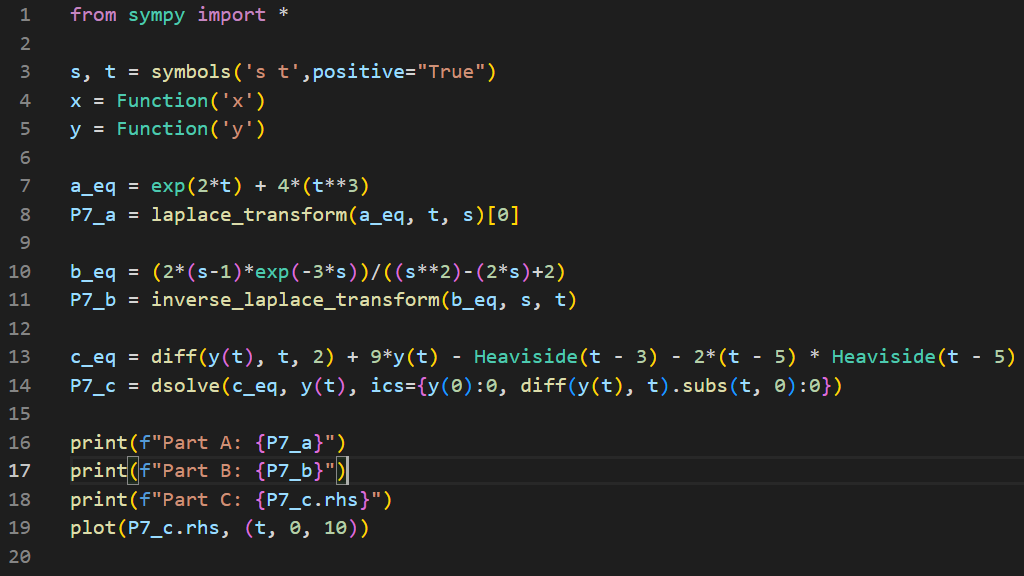
\includegraphics[width=0.8\textwidth]{Images/p7 code.png}

\includegraphics[width=0.6\textwidth]{Images/p7 graph.png}

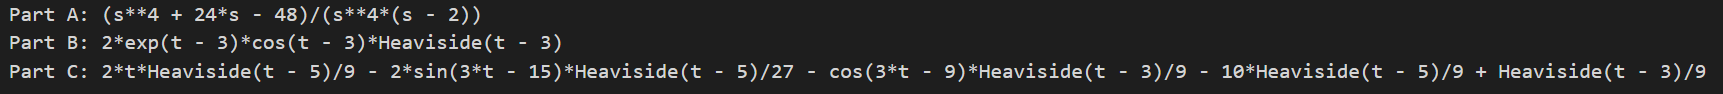
\includegraphics[width=1\textwidth]{Images/p7 answers.png}

\end{document}